\section{Ausgabem�glichkeiten}

\hypertarget{cmd:datei-drucken}{}
\hypertarget{cmd:datei-seitenansicht}{}
\hypertarget{cmd:datei-druckereinrichtung}{}
\subsection{Drucken}

Erstellte Karten k�nnen auf einem Drucker /
Plotter zu Papier gebracht werden. Die Druckerauswahl sowie die Drucker-Einstellungen erfolgen �ber den Men�punkt \menu{Druckereinrichtung} im Dateimen� (Abb. \ref{fig:seitenansicht}). 
In der Seitenansicht besteht die M�glichkeit, die Formatierung und Anordnung der dargestellten Elemente zu ver�ndern.\\
\\
\begin{figure}[hbtp]
	\begin{center}
		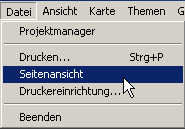
\includegraphics[scale=0.60]{seitenansicht}
	\end{center}
	\caption{Auswahl der Seitenansicht}
	\label{fig:seitenansicht}
\end{figure}


Elemente, die im Layout verf�gbar sind:
\begin{itemize}
	\item{Karte}
	\item{Projekt�berschrift}
	\item{Legende}
	\item{Textfeld}
	\item{Logo}
\end{itemize}

\begin{figure}[hbtp]
	\begin{center}
		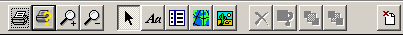
\includegraphics[scale=0.50]{toolleiste}
	\end{center}
	\caption{verf�gbare Aktionsbuttons f�r die Layoutgestaltung}
	\label{fig:toolleiste}
\end{figure}

In der Seitenansicht k�nnen diese Elemente hinzugef�gt, ge�ndert oder wieder entfernt werden. Dies betrifft sowohl die Projekt�berschrift (Abb.~\ref{fig:texteigenschaften}) als auch die Legende (Abb.~\ref{fig:legendeeigenschaften}). Das Element "`Firmenlogo"' (Abb.~\ref{fig:logofestlegen}) dient zur Platzierung einer Grafik-Datei im bitmap-Format z.B. im Zusammenhang mit einem Firmenstempel. Bei Textfeldern k�nnen Sie beliebigen Absatz-Text eingeben und diesen entsprechend formatieren (Abb.~\ref{fig:toolleiste}).
In der Legende werden nur die im Kartenfenster als sichtbar markierten Themen angezeigt. Um Themen  im Plot hinzuzuf�gen oder zu entfernen, m�ssen diese zun�chst in der Kartenansicht aktiviert bzw. deaktiviert werden.\\


\begin{figure}[hbtp]
	\begin{center}
		\includegraphics[scale=0.60]{legendeeigenschaften}
	\end{center}
	\caption{�ndern der Legende}
	\label{fig:legendeeigenschaften}
\end{figure}

\begin{figure}[hbtp]
	\begin{center}
		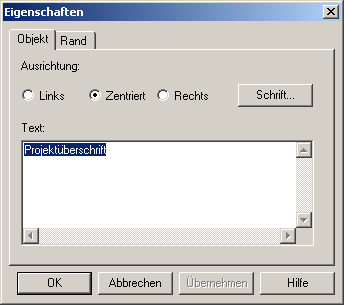
\includegraphics[scale=0.50]{texteigenschaften}
	\end{center}
	\caption{Texte eingeben oder �ndern}
	\label{fig:texteigenschaften}
\end{figure}

\begin{figure}[hbtp]
	\begin{center}
		
\includegraphics[scale=0.50]{logo}
	\end{center}
	\caption{Logo festlegen}
	\label{fig:logofestlegen}
\end{figure}


\subsubsection{Ausgabema�stab festlegen}
Die �nderung des Ausgabe-Ma�stabes ist mittels eines Doppelklicks auf das Kartenelement m�glich. Hier bestehen 2 Optionen:\\


\paragraph{Kartenausschnitt anpassen:}
\label{sec:KartenausschnittAnpassen}
Sie k�nnen den Kartenausschnitt an den neuen Ma�stab anpassen, d.h. es wird nur die Darstellung innerhalb des Kartenelemts gem�ss des von Ihnen gew�hlten Ma�stabs ge�ndert; die Gr��e des Kartenelemts selbst wird beibehalten.

\paragraph{Druckbereich anpassen:}
\label{sec:DruckbereichAnpassen}
\ In diesem Fall wird das Kartenelement und dementsprechend auch der Druckbereich an den vorgegebenen Ma�stab angepasst und erm�glicht z.B. eine ma�stabsgetreue Ausgabe im Grossformat
oder auf mehreren Ausgabebl�ttern.

\begin{figure}[hbtp]
	\begin{center}
		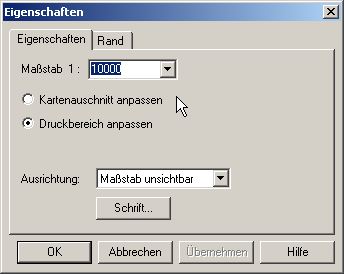
\includegraphics[scale=0.50]{massstab}
	\end{center}
	\caption{Ma�stab w�hlen}
	\label{fig:massstab}
\end{figure}

\begin{figure}[hbtp]
	\begin{center}
% KAPUTT!
%		\includegraphics[scale=0.40]{ausgabemoeg_preview}
	\end{center}
	\caption{Seitenansicht des Kartenfensters}
	\label{fig:ausgabemoeg_preview}
\end{figure}
%Abb.24: Seitenansicht des Kartenfensters\\

Zur Ausgabe der Karte dient das Druckersymbol. Die Karte wird mit den
vorgegebenen Druckereinstellungen - wie aus anderen Windows-Anwendungen
gewohnt - gedruckt.

\hypertarget{cmd:karte-exportierenals}{}
\hypertarget{cmd:karte-inzwischenablage}{}
\subsection{Bild speichern}
Im \wspmap\ besteht die M�glichkeit, die auf dem Bildschirm dargestellte Karte entweder als Bitmap (*.bmp) oder als EMF-Bilddatei (*.emf) zu exportieren \menu{Karte / Exportieren als}. Damit steht die erzeugte Karte f�r die Weiterverarbeitung mit anderen Anwendungen oder zur Einbindung in ein Text-Dokument zur Verf�gung.  
